\documentclass{article}
\usepackage{tikz}
\usepackage{amsmath}
\usetikzlibrary{calc,patterns,angles,quotes}
\begin{document}

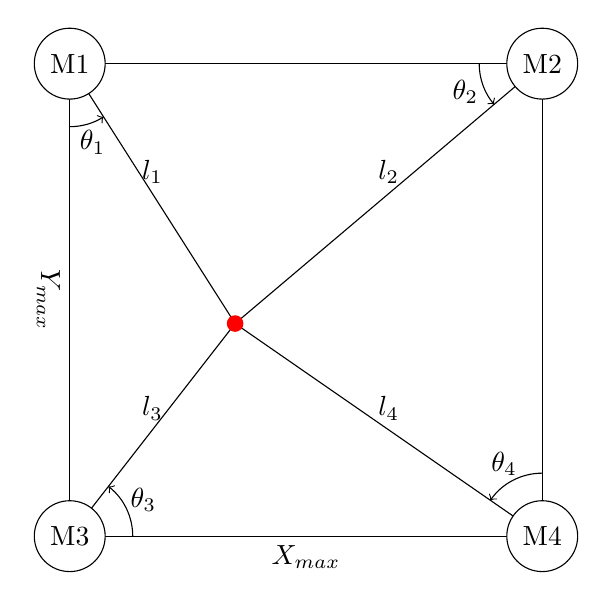
\begin{tikzpicture}[scale=1.5]

\draw (0,0) -- (4,0) node[midway,below] {$X_{max}$} -- (4,4) -- (0,4) -- cycle node[midway,below,sloped] {$Y_{max}$}  ;

\coordinate (M1) at (0,4);
\coordinate (M2) at (4,4);
\coordinate (M3) at (0,0);
\coordinate (M4) at (4,0);
\coordinate (c) at (1.4, 1.8);
\draw (c) -- (0,0) node[midway,above] {$l_3$} ;
\draw (c) -- (0,4) node[midway,above] {$l_1$} ;
\draw (c) -- (4,0) node[midway,above] {$l_4$} ;
\draw (c) -- (4,4) node[midway,above] {$l_2$} ;
%\draw ()
\fill[red] (c) circle (2pt);

\draw[fill=white] (M3) circle (0.3cm) node[text=black] {M3};

\draw[fill=white] (M1) circle (0.3cm) node[text=black] {M1};

\draw[fill=white] (M4) circle (0.3cm) node[text=black] {M4};

\draw[fill=white] (M2) circle (0.3cm) node[text=black] {M2};

\pic [draw, angle radius=0.8cm, ->, "$\theta_1$", angle eccentricity=1.3] {angle = M3--M1--c};

\pic [draw, angle radius=0.8cm, ->, "$\theta_2$", angle eccentricity=1.3] {angle = M1--M2--c};

\pic [draw, angle radius=0.8cm, ->, "$\theta_4$", angle eccentricity=1.3] {angle = M2--M4--c};

\pic [draw, angle radius=0.8cm, ->, "$\theta_3$", angle eccentricity=1.3] {angle = M4--M3--c};

\end{tikzpicture}
\linebreak

Inverse Kinematics:
\begin{equation}
\cos(\theta_3) = \frac{X_{max}{}^2 + l_3{}^2 - l_4{}^2}{2*X_{max}*l_3}
\end{equation}
\begin{equation}
X = l_3\sin(\theta_3)
\end{equation}
\begin{equation}
Y = l_3\cos(\theta_3)
\end{equation}

%Or, without trigonometry:

\begin{equation}
X = \left(\frac{X_{max}{}^2 + l_3{}^2 - l_4{}^2}{2*X_{max}*l_3}\right) = \frac{X_{max}}{2} + \frac{l_3{}^2 - l_4{}^2}{2*X_{max}}
\end{equation}

\begin{equation}
Y = \left(\frac{Y_{max}{}^2 + l_4{}^2 - l_1{}^2}{2*Y_{max}*l_3}\right) = \frac{Y_{max}}{2} + \frac{l_3{}^2 - l_4{}^2}{2*Y_{max}}
\end{equation}

Forward Kinematics:
\begin{equation}
l_1 = \sqrt{\left(X_{max}-X\right)^2 + \left(Y_{max}-Y\right)^2}
\end{equation}

\begin{equation}
l_2 = \sqrt{\left(X\right)^2 + \left(Y_{max}-Y\right)^2}
\end{equation}

\begin{equation}
l_3 = \sqrt{\left(X\right)^2 + \left(Y\right)^2}
\end{equation}

\begin{equation}
l_4 = \sqrt{\left(X_{max}-X\right)^2 + \left(Y\right)^2}
\end{equation}
\newpage
\begin{equation}
\begin{aligned}
M1 = Y - X \\
M2 = Y + X\\
M3 = -Y -X\\
M4 = -Y + X\\
\end{aligned}
\end{equation}


\end{document}